%%%%%%%%%%%%%%%%%%%%%%%%%%%%%%%%%%%%%%%%%%%%%%%%%%%%%%%%%%%%%%%%%%%%%%%%%%%%%%%%%%%%%%%%%%%%%%%%%%%%%%%%%%%%%%%%%%%%%%%%%%%%%%%%%%%%%%%%%%%%%%%%%%%%%%%%%%%
% This is just an example/guide for you to refer to when submitting manuscripts to Frontiers, it is not mandatory to use Frontiers .cls files nor frontiers.tex  %
% This will only generate the Manuscript, the final article will be typeset by Frontiers after acceptance.   
%                                              %
%                                                                                                                                                         %
% When submitting your files, remember to upload this *tex file, the pdf generated with it, the *bib file (if bibliography is not within the *tex) and all the figures.
%%%%%%%%%%%%%%%%%%%%%%%%%%%%%%%%%%%%%%%%%%%%%%%%%%%%%%%%%%%%%%%%%%%%%%%%%%%%%%%%%%%%%%%%%%%%%%%%%%%%%%%%%%%%%%%%%%%%%%%%%%%%%%%%%%%%%%%%%%%%%%%%%%%%%%%%%%%

%%% Version 3.4 Generated 2022/06/14 %%%
%%% You will need to have the following packages installed: datetime, fmtcount, etoolbox, fcprefix, which are normally inlcuded in WinEdt. %%%
%%% In http://www.ctan.org/ you can find the packages and how to install them, if necessary. %%%
%%%  NB logo1.jpg is required in the path in order to correctly compile front page header %%%

\documentclass[utf8]{FrontiersinHarvard} % for articles in journals using the Harvard Referencing Style (Author-Date), for Frontiers Reference Styles by Journal: https://zendesk.frontiersin.org/hc/en-us/articles/360017860337-Frontiers-Reference-Styles-by-Journal
%\documentclass[utf8]{FrontiersinVancouver} % for articles in journals using the Vancouver Reference Style (Numbered), for Frontiers Reference Styles by Journal: https://zendesk.frontiersin.org/hc/en-us/articles/360017860337-Frontiers-Reference-Styles-by-Journal
%\documentclass[utf8]{frontiersinFPHY_FAMS} % Vancouver Reference Style (Numbered) for articles in the journals "Frontiers in Physics" and "Frontiers in Applied Mathematics and Statistics" 

%\setcitestyle{square} % for articles in the journals "Frontiers in Physics" and "Frontiers in Applied Mathematics and Statistics" 
\usepackage{url,hyperref,lineno,microtype,subcaption,siunitx,todonotes,fixltx2e}
\usepackage[onehalfspacing]{setspace}

\linenumbers


% Leave a blank line between paragraphs instead of using \\


\def\keyFont{\fontsize{8}{11}\helveticabold }
\def\firstAuthorLast{Humble} %use et al only if is more than 1 author
\def\Authors{James Humble\,$^{1}$}
% Affiliations should be keyed to the author's name with superscript numbers and be listed as follows: Laboratory, Institute, Department, Organization, City, State abbreviation (USA, Canada, Australia), and Country (without detailed address information such as city zip codes or street names).
% If one of the authors has a change of address, list the new address below the correspondence details using a superscript symbol and use the same symbol to indicate the author in the author list.
\def\Address{$^{1}$Randolph, MA, USA}
% The Corresponding Author should be marked with an asterisk
% Provide the exact contact address (this time including street name and city zip code) and email of the corresponding author
\def\corrAuthor{James Humble}

\def\corrEmail{james.m.d.humble@gmail.com}




\begin{document}
\onecolumn
\firstpage{1}

\title[Resource-dependent heterosynaptic plasticity]{Resource-dependent heterosynaptic spike-timing-dependent plasticity in recurrent networks}

\author[\firstAuthorLast ]{\Authors} %This field will be automatically populated
\address{} %This field will be automatically populated
\correspondance{} %This field will be automatically populated

\extraAuth{}% If there are more than 1 corresponding author, comment this line and uncomment the next one.
%\extraAuth{corresponding Author2 \\ Laboratory X2, Institute X2, Department X2, Organization X2, Street X2, City X2 , State XX2 (only USA, Canada and Australia), Zip Code2, X2 Country X2, email2@uni2.edu}


\maketitle
Number of words: 3331\\
Number of figures: 4\\
Number of tables: 0%
\vspace{25px}

\begin{abstract}
%%% Leave the Abstract empty if your article does not require one, please see the Summary Table for full details.
\section{}
Many computational models that incorporate spike-timing-dependent plasticity (STDP) have shown the ability to learn from stimuli, supporting theories that STDP is a sufficient basis for learning and memory. However, to prevent runaway activity and potentiation, particularly within recurrent networks, additional global mechanisms are commonly necessary. A STDP-based learning rule, which involves local resource-dependent potentiation and heterosynaptic depression, is shown to enable stable learning in recurrent spiking networks. A balance between potentiation and depression facilitates synaptic homeostasis, and learned synaptic characteristics align with experimental observations.
\tiny
 \keyFont{ \section{Keywords:} spike-timing-dependent plasticity, homeostasis, recurrent network, spiking, learning, plasticity, heterosynaptic, XXXXXXXKEYWORDXXXXXXXXX} %All article types: you may provide up to 8 keywords; at least 5 are mandatory.
\end{abstract}
\section{Introduction}
The concept of spike-timing-dependent plasticity (STDP) has been thoroughly researched and frequently serves as a foundation for learning in computational models. Various studies adopt STDP in diverse formats. For instance, it may be utilized with either an additive or a multiplicative rule for updates: Potentiation or depression may depend on or be independent of a synapse's weight. Different STDP implementations can lead to varied outcomes, with some rules more closely reflecting phenomena observed in experiments. These variations include 1) synaptic weight distributions, 2) the presence of nonpotentiable synapses, 3) silent synapses, 4) synaptic persistence, and 5) competition between synapses:

\begin{enumerate}
    \item Empirically identified synaptic weight distributions generally display a uni-modal pattern that peaks close to zero, characterized by numerous weak synapses and a few strong connections forming a long tail \citep{Buzsaki.2004n8e,Yasumatsu.2008g4n,KASAI.20239m}. In computational models, synaptic distributions change based on whether STDP is implemented additively or multiplicatively. In feedforward networks, additive STDP often produces bi-modal distributions, with peaks located near zero and the upper limit of synaptic weight \citep{Rossum.2000jye,Barbour.2007,Morrison.2008}. In contrast, multiplicative STDP often generates uni-modal distributions with a peak situated between zero and the upper bound \citep{Rossum.2000jye,Barbour.2007,Morrison.2008}. In recurrent networks, additive STDP can produce a uni-modal distribution with a peak at the upper-bound and multiplicative, uni- or multi-modal distributions \citep{Morrison.2007}.

    \item Silent synapses are primarily defined by their absence of $\alpha$-amino-3-hydroxy-5-methyl-4-isoxazolepropionic acid (AMPA) receptors, as comprehensively discussed by Montgomery and colleagues \citeyearpar{Montgomery.2004}. Despite the scarcity of AMPA receptors, these synapses often retain a degree of plasticity due to the presence of \textit{N}-methyl-D-aspartate (NMDA) receptors \citep{Kim.2025}. In a study by Brunel et al.~\citeyearpar{Brunel.2004}, a prominent and sharply delineated subset of silent synapses was integrated into an empirically derived distribution by assessing those potentially undetected because of technological limitations and their deficiency in AMPA receptors. Such a peak is observed in spine volume \citep{Yasumatsu.2008g4n} and synaptic efficacy \citep{Barbour.2007}.

    \item Research has indicated that certain synapses may not be capable of potentiation. For instance, Debanne et al.~\citeyearpar{Debanne.1999} reported the inability to induce potentiation in \SI{24}{\percent} of the synapses examined. The authors propose that this nonpotentiability might be attributed to synapses individually reaching saturation. Conversely, computational models often employ either a universal upper limit across all synapses or a global normalizing mechanism and neglecting these constraints may lead to excessive activity and potentiation \citep{Rossum.2000jye}.

    \item The persistence of synapses is typically considered to be fundamentally important for memory. In their study, Billings et al.~\citeyearpar{Billings.2009} investigated the durability of synaptic weights governed by STDP principles and found that additive STDP facilitates stability, whereas multiplicative STDP causes instability due to rapid weight variations. Empirical evidence from long-term potentiation (LTP) studies indicates a two-phase persistence: an initial phase that diminishes swiftly and seems to be reliant on neuronal activity \citep{Dong.2015}, and a later phase capable of sustaining LTP over prolonged periods, possibly extending to a year \citep{Abraham.2002}. There is, however, strong evidence demonstrating that spine volumes fluctuate in the absence of activity and plasticity (reviewed by Kasai \citeyearpar{KASAI.20239m}) and that such fluctuations combined with STDP can be stable \citep{Humble.2019}. In this case, the mean spine volume of a group of neurons must be persistent rather than the individual synaptic strengths.

    \item Whereas STDP following an additive rule is known for its strong competitive interactions, STDP governed by a multiplicative rule typically exhibits limited competition, prompting the incorporation of supplementary mechanisms such as synaptic scaling or intrinsic fluctuations to achieve the competition essential for learning \citep{Rossum.2000jye,Humble.2019}. The inherently competitive aspect of additive STDP typically necessitates enforcing a stringent upper limit on synaptic strength to control excessive potentiation. In contrast, multiplicative STDP operates under more flexible upper limits determined by weight dependency. A drawback of deploying global limits is their assignment of preset values before the learning process, which may not align with biological realism. Moreover, as mentioned above, Debanne et al.~\citeyearpar{Debanne.1999} demonstrated the possibility of individual synaptic upper limits.
\end{enumerate}

Furthermore, to control runaway activity, mechanisms such as synaptic scaling \citep{Turrigiano.2008}, inhibition \citep{Bannon.2020,Eckmann.2024}, or the Beinenstock-Cooper-Munro rule \citep{Cooper.2012} are typically included with Hebbian-based learning rules in recurrent networks. However, these can operate on a slower timescale than STDP.

The above picture is further complicated by experiments showing that heterosynaptic plasticity can occur at unstimulated spines near a stimulated one (reviewed by Chater and Goda \citeyearpar{Chater.2021}). Essentially, given some homosynaptic activity in a subset of spines, heterosynaptic changes have been observed at unstimulated ones. The distance dependence and direction of these heterosynaptic changes are potentially competitive \citep{Chater.2024}.

Motivated by these experimental results, this paper explores ongoing research into computational disparities by utilizing a learning methodology that integrates `resources' alongside heterosynaptic plasticity in a spiking recurrent network. In a computational model of individual neurons \citep{Chen.201381r} and a feedforward network (Chapter 5 of \citep{Humble.2013}), it has previously been shown that heterosynaptic plasticity can be beneficial in controlling activity and plasticity.

In addition to networks with static connectivity, progressive loss of synapses is a hallmark of many neurodegenerative diseases, including Huntington's, Parkinson's, and Alzheimer's \citep{Herms.2015,Meftah.2023}, and neuropsychiatric disorders such as schizophrenia and depression \citep{Penzes.2011}. To counteract synaptic loss, the existence of compensatory mechanisms has been suggested that include enlargement of the remaining spines and increased spinogenesis \citep{Bhembre.2023}.

By advancing STDP through the incorporation of limited resources for potentiation and merging it with heterosynaptic depression that affects neighboring synapses, the results reveal that this model effectively resolves the discrepancies mentioned above while presenting an innate mechanism for both synaptic homeostasis and neurodegenerative compensation.

\section{Methods}
The network structure, Fig.~\ref{figs:methods:network}, consists of a pool of $N_{\mathrm{exc}}=\SI{200}{}$ excitatory neurons recurrently connected with plastic excitatory synapses with a probability of \SI{25}{\percent}. Independent Poisson spike trains are presented to the pool with an input connection probability of \SI{10}{\percent} from $N_{\mathrm{in}}=\SI{50}{}$ spike trains. All connections have axonal delays drawn from a uniform distribution from \SI{1}{\milli\second} to \SI{5}{\milli\second} \citep{Lemarechal.2021yt1}.

Excitatory neurons are refractory leaky integrate-and-fire cells, Eqs.~\ref{eqs:methods:LIF}. The membrane potential of each neuron, $v$, follows low-pass dynamics with a time constant $\tau_{v}=\SI{25}{\milli\second}$ \citep{Rall.1969w7} and is reset when it reaches the firing threshold, $\theta=\SI{1}{}$, Fig.~\ref{figs:methods:neurons_and_synapses} bottom.

\begin{subequations}
    \begin{gather}
        \tau_{v} \frac{dv}{dt}= -v + r ( \sum_{i}^{N_{\mathrm{in}}}{s_{i}} + \sum_{j}^{N_{\mathrm{exc}}}{s_{j}} ) \\
        V \rightarrow 0 \qquad \mbox{if } V \geq \theta
    \end{gather}
    \label{eqs:methods:LIF}
\end{subequations}

An absolute refractory period of \SI{3}{\milli\second} is followed by a relative refractoriness period, $\tau_{r}=\SI{5}{\milli\second}$, Eq.~\ref{eqs:methods:refractoriness} and Fig.~\ref{figs:methods:neurons_and_synapses} middle.

\begin{equation}
    \tau_{r} \frac{dr}{dt}= 1-r
    \label{eqs:methods:refractoriness}
\end{equation}

All input and recurrent afferents were modeled as synaptic currents, $s^{\prime}$ and $s$, Eqs.~\ref{eqs:methods:alpha} and Fig.~\ref{figs:methods:neurons_and_synapses} top. $\tau_{sr}=\SI{2.6}{\milli\second}$ is the time constant for the synaptic current rise and $\tau_{sf}=\SI{31.3}{\milli\second}$ the decay constant \citep{Hunt.2022}. The input of each synapse consists of binary neuron spikes, $I_{i}$, scaled by the synapse's weight, $w_{i}$.

\begin{subequations}
    \begin{gather}
        \tau_{sr} \frac{ds^{\prime}}{dt}= -s^{\prime} + I \text{ } w \\
        \nonumber \\
        \tau_{sf} \frac{ds}{dt}= -s+s^{\prime}
    \end{gather}
    \label{eqs:methods:alpha}
\end{subequations}
%
Pairs of presynaptic and postsynaptic spikes evoke changes in synaptic weight, $\Delta w=f(\tau)$, given as a function of their temporal distance, $\tau=\textit{post-spike time}-\textit{pre-spike time}$, Fig.~\ref{figs:methods:STDP}. Equation \ref{eqs:methods:expSTDP} describes the STDP function used,  where $\tau_{STDP}=\SI{20}{\milli\second}$ \citep{Bi.1998}. Depression is weight dependent, as observed by Bi and Poo \citeyearpar{Bi.1998}, Fig.~\ref{figs:methods:weight_dependence}. Recurrent weights were bounded $[0, +\infty)$. See below for a description of the inclusion of \SI{0.18}{} in depression.

\begin{equation}
    f(\tau) = 	\begin{cases}
                    \mathrm{exp} \left (%
                    \frac{-\tau}{\tau_{STDP}} \right ) & \mbox{if } \tau \geq 0 \\ \\
                    0.18 \text{ } \mathrm{exp} \left (%
                    \frac{\tau}{\tau_{STDP}} \right ) \text{ } w & \mbox{if } \tau < 0
                \end{cases}
    \label{eqs:methods:expSTDP}
\end{equation}

The initial input weights are set with random values drawn from a uniform distribution between \SI{0}{} and \SI{1}{}. All recurrent weights, $w$, are initially assigned \SI{0}{} as akin to a newly formed network.

This typical STDP implementation is extended as in Humble \citeyearpar{Humble.2013} to include the requirement of resources for potentiation paired with potentiation-driven heterosynaptic depression in neighboring synapses. Firstly, a pool of resources is included, $p$. Similarly to many receptors and proteins that undergo degradation or recycling, the pool's resources decay with a time constant of $\tau_{p}=\SI{10}{\second}$, Eq.~\ref{eqs:methods:rbSTDPpool}.

\begin{equation}
    \tau_{p} \frac{dp}{dt}= -p
    \label{eqs:methods:rbSTDPpool}
\end{equation}

The amounts of the initial resource pool are assigned by Eq.~\ref{eqs:methods:rbSTDPpoolInitial} where $\xi$ is a random number from a standard normal distribution. The constant multiple was found through a parameter search to ensure that the weights were strong enough that the activity continued after stimulation stopped. A lognormal distribution is chosen as skewed distributions are observed for many aspects of brain dynamics \citep{Buzsaki.2014}.

\begin{equation}
    2 \text{ } e^{\xi}
    \label{eqs:methods:rbSTDPpoolInitial}
\end{equation}

When updating the weights with resource-dependent STDP, there are three scenarios, Fig.~\ref{figs:methods:rbSTDP}:

\begin{itemize}
    \item When potentiating a synapse, its neighbors are actively depressed by an exponential function of their distance to the potentiating synapse, and the potentiating amount to a maximum distance of \SI{3}{} synapses.

    \item When a potentiating synapse and its neighbors have no resources left, the potentiating synapse acquires resources from the pool, if available.

    \item When a synapse is depressed, its resources are relocated to the pool for reuse.
\end{itemize}

For simplicity, time constants for resource mobility are neglected; hence, resources can transfer between a synapse and the pool, and vice versa, within a single time step. See Chapter 5 of Humble \citeyearpar{Humble.2013} for pseudo-code.

With local heterosynaptic plasticity, depression dominates because potentiation events are accompanied by depression, and thus depression has to be decreased. It has previously been found that \SI{0.18}{} was a suitable multiple for depression such that potentiation and depression were balanced \citep{Humble.2013}. This reduced depression, Fig.~\ref{figs:methods:STDP}, matches the experimental observations of decreased depression relative to potentiation \citep{Bi.1998}.

The rate of the input spike trains is \SI{50}{\hertz} for the first \SI{30}{\second}, Fig.~\ref{figs:methods:stimulation_protocol}.

All simulations used forward Euler integration with a time step of $dt=\SI{0.1}{\milli\second}$ and were implemented in MATLAB.

\section{Results}
During stimulation of a typical network, most neurons in the excitatory pool fire with increased firing rates, Figs.~\ref{figs:results:firing_rate} and \ref{figs:results:firing_rate_sorted}. After stimulation, a subset continues to fire representing a learned memory. Not all neurons are recruited into the memory, due to initial random input and recurrent connectivity and random activity-driven plasticity. Furthermore, after learning, the firing rates of many neurons change, Fig.~\ref{figs:results:firing_rate_change}; nevertheless, the memory is preserved.

After learning, weight statistics match those found experimentally---five observations were identified in the introduction:

\begin{enumerate}
    \item Similarly to the feedforward model studied by Humble \citeyearpar{Humble.2013}, the weight distribution for recurrent connections at the end of the simulation is unimodal, Fig.~\ref{figs:results:weight_distribution}, matching those observed experimentally (see supplementary materials Fig.~1 for additive and multiplicative STDP results in this model.)

    \item The distribution also shows a large peak of empty synapses: silent synapses.

    \item Resource-based STDP endows reduced and nonpotentiability, Fig.~\ref{figs:results:non_potentiable}. Specifically, the actual potentiation amount as a percentage of that determined by the STDP window function demonstrates that sometimes not enough resources are available to fully potentiate a synapse; some times very little or no potentiation was observed.

    \item Resource-based STDP is stable, with weights remaining persistent in a longer simulation, Fig.~\ref{figs:results:long}.

    \item Related to the weight distribution, Humble \citeyearpar{Humble.2013} found that weights converge to individual upper bounds. This is also the case in the recurrent network despite the positive feedback loop present due to plasticity. It was observed that weights reach their own saturation points, Fig.~\ref{figs:results:weights_traces}. Furthermore, due to the distance dependence of heterosynaptic depression, analysis indicates that resource-based heterosynaptic STDP promotes synaptic sparsity and synaptic competition for limited resources, with functional spines becoming spatially distributed along the dendrite. The average distance between a nonfilopodia spine and its nearest nonfilopodia spine neighbor increases during learning, Fig.~\ref{figs:results:weights_distance}.
\end{enumerate}

Most of the resources available in the neurons' pools quickly decrease due to plasticity driven changes, Fig.~\ref{figs:results:resource_pools}. Some pools may not be used up due to plasticity and instead naturally decay.

During the initial learning phase, the network's in/out degree increases and stabilizes $\approx\SI{3}{}$, and the closeness (where the length of the paths is the axonal delay) decreases, Fig.~\ref{figs:results:centrality}. The decrease in closeness demonstrates that learning optimizes for short delays. After the initial learning phase, the network is further optimized with an additional increase in nonfilopodia spine distance and a decrease in closeness.

Furthermore, the network structure changes during this optimizing phase with weights either increasing or decreasing: Figs.~\ref{figs:results:network_after_learning} to \ref{figs:results:network_end}. Most strong connections are stable with a few changing; the majority of optimization changes are with weaker synapses. However, most synapses do not change. These changes may be the basis for the observation that only a subset of neurons continue to fire after learning.

These results in a typical network demonstrate that resource-based STDP is capable of stable learning in recurrent networks with an innate homeostasis mechanism controlling runaway activity and potentiation. Next, to model spine loss in neurodegenerative diseases, synapses are progressively removed, Figs.~\ref{figs:results:AD:stimulation_protocol} and \ref{figs:results:AD:connections}.

In a typical network with resource-based heterosynaptic STDP, the memory is maintained until $\approx\SI{17}{\percent}$ of the original connections remain, Figs.~\ref{figs:results:AD:firing_rate}. As synapses are removed, their resources replenish the pool and allow further compensatory potentiation with an increase in mean synaptic weight and transient increases in the pool of resources, Figs.~\ref{figs:results:AD:weights_traces} and \ref{figs:results:AD:resource_pools}. However, when this replenishment is blocked, the memory is only maintained until $\approx\SI{72}{\percent}$ synapses remain, Figs.~\ref{figs:results:AD:Hz_no_resources}---with no increase in the remaining synaptic weights, Fig.~\ref{figs:results:AD:weights_traces_no_resources}.

This is further illustrated when comparing the sum of weights as a percentage of the maximum sum, Fig.~\ref{figs:results:AD:weights_sums}. Under the replenishment-blocking condition, the total synaptic input disappears $\approx\SI{4}{}$ times faster than under the control condition. Moreover, loss of neuron activity is sudden without replenishment of resources; whereas with replenishment of resources there is a progressive loss, Fig.~\ref{figs:results:AD:Hz_sums}.

\section{Discussion}
Discrepancies were reconciled between computational STDP models and empirical observations by using a STDP framework based on resource-dependent heterosynaptic STDP in a recurrent spiking network. By integrating resource-dependent potentiation with heterosynaptic depression at nearby synapses, neurons performed a learning task while preserving synaptic weight attributes and statistical traits consistent with biological data.

Resource-dependent heterosynaptic STDP results in weight distributions characterized by a singular peak and a pronounced tail. The distribution also shows a large peak at zero of spines empty of resources (silent synapses) similar to those estimated by Brunel et al.~\citeyearpar{Brunel.2004} and similar to an abundance of filopodia as seen by Yasumatsu et al.~\citeyearpar{Yasumatsu.2008g4n} and reviewed by Kasai \citeyearpar{KASAI.20239m}.

Furthermore, this approach to heterosynaptic STDP incorporates robust competitive dynamics and synaptic homeostasis, leading to varying intrinsic upper limits for individual synapses at which a synapse is no longer potentiable. In addition, the STDP rule promotes sparse spatial encoding in afferents and therefore strong competition between neighboring spines for limited resources. This homeostasis among weights is independent of any additional normalization mechanism or universal constraints to regulate learning. Such synaptic homeostasis is a compelling mechanism for stabilizing neural activity and plasticity within recurrent networks.

Finally, given progressive synaptic loss, resource-based STDP demonstrated an innate compensatory mechanism due to replenishment of resources; this mechanism has been hypothesized to counteract a loss in input \citep{Bhembre.2023}. Loss of synaptic input is associated with early stages of neurodegenerative diseases, for example, Alzheimer's disease \citep{Spires.2005}. Resource-based STDP demonstrated the ability to maintain total synaptic input by replenishing resources in the pool after synaptic removal. Moreover, resource-based STDP demonstrated a sufficient substrate for observations showing enlargement of synapses following insults such as deafferentation and sensory deprivation \citep{Chen.1982,Barnes.2017d2} and the hypothesized spine enlargement in Alzheimer's disease \citep{Bhembre.2023}. Finally, resource-based STDP exhibited a progressive loss in, rather than a sudden loss in, neuron activity. How this relates to aberrant activity observed in Alzheimer's disease \citep{Korzhova.2021} is unknown, and exploring this offers an interesting future extension to this work.

Given that the proposed STDP rule aligns with experimentally observed weight statistics and supports hypothesized neurodegenerative compensatory mechanisms, its potential biological plausibility warrants examination. Royer et al.~\citeyearpar{Royer.2003} observed in amygdala slices that the induction of long-term depression (potentiation) resulted in corresponding long-term potentiation (depression) at distally located dendritic sites, determined by the distance from the initial induction site. In contrast, Hou et al.~\citeyearpar{Hou.2008} reported no such synaptic changes at adjacent sites in cultured hippocampal neurons derived from rat embryos.

The research carried out by Oh et al.~\citeyearpar{Oh.2015} in P6-P7 hippocampal slice cultures aligns with our STDP model. Stimulation-induced potentiation in specific spines was demonstrated to cause a reduction in the size of adjacent unstimulated spines. This observation can be explained by two potential mechanisms: first, the competition among nearby spines for a scarce resource, or second, an activity-triggered signal facilitating the reduction of adjacent spines. The findings of Oh et al.~lend credence to the second hypothesis. They determined that blocking calcineurin, IP\textsubscript{3} receptors or group I metabotropic glutamate receptors hinders heterosynaptic shrinkage, without affecting the potentiation process when Ca\textsuperscript{2+}/calmodulin-dependent protein kinase II (CaMKII) is inhibited. This evidence indicates that synaptic potentiation and the associated decrease in nearby synaptic strength operate through distinct pathways.

Bian et al.~\citeyearpar{Bian.2015} observed that competition among spines for cadherin/catenin complexes plays a crucial role in orchestrating both the maturation of individual spines and the pruning of adjacent spines. Their \textit{in vivo} studies revealed that variations in cadherin/catenin complex concentrations between neighboring spines lead to a redistribution of $\beta$-catenin, which in turn influences whether a spine matures or is trimmed. Crucially, they demonstrated that this process depends on neuronal activity and the distance between the enlarging spine and the nearby one that is slated for elimination. Additionally, this competitive mechanism was not restricted to individual neurons; it occurred across neighboring neurons receiving similar axonal inputs.

Within the framework of long-term potentiation (LTP), the relocation of AMPA receptors to synaptic sites is associated with increased synaptic activity \citep{Hayashi.2000,Sutton.2006u4b,Shi.2001}. In this process, CaMKII experiences autophosphorylation when intracellular Ca\textsuperscript{2+} levels rise through NMDA receptor-mediated channels, culminating in the phosphorylation of GluR1 \citep{Roche.1996}. AMPA receptors can originate from multiple sources, such as recycling endosomes \citep{Park.2004} and the trans-Golgi network \citep{Horton.2004}. Our model consolidates these different origins into a common pool, taking advantage of evidence that AMPA receptors can traverse long distances, facilitated by movement along dendritic membranes \citep{Choquet.2003} and microtubule pathways \citep{Washbourne.2002}. Regarding the mechanism that underlies heterosynaptic depression, Oh et al. \citeyearpar{Oh.2015} observed that blocking calcineurin, IP\textsubscript{3}Rs, or group I metabotropic glutamate receptors hindered the contraction of adjacent spines. Additionally, Bian et al.~\citeyearpar{Bian.2015} propose the existence of a single molecular structure that fulfills dual roles, both as a `resource' and as a transmitter of depressive signals. Finally, recent experimental and computational evidence suggests that Ca\textsuperscript{2+} activity is a key component of competitive heterosynaptic plasticity \citep{Chater.2024}.

The depiction of STDP herein does not include explicit modeling of biological signaling pathways or diffusible molecules that might cause depression in neighboring synapses after activity-driven potentiation, nor does it specify a precise timeline for such processes. Furthermore, it does not incorporate the transfer of resources into or out of a dendritic spine. Introducing these complexities could impose interesting limitations on the model, suggesting areas for future investigation.

Although a precise `resource' is not identified, nor is a specific depression signal characterized, multiple hypotheses suitable for experimental examination can be proposed under healthy and neurodegenerative conditions.

\begin{itemize}
    \item As described by Oh and colleagues \citeyearpar{Oh.2015}, suppressing the heterosynaptic depression signal could allow learning driven by potentiation under healthy conditions to continue until resources in the pool(s) are exhausted. Subsequent learning would require the creation of new resources. As a result, while the pace of learning may reduce under signal-suppressed conditions compared to when active signals are present, it would not come to a complete stop until all resources are used with no change in neighboring spines. 
    
    \item Suppression of the depression signal under neurodegenerative conditions might interfere with memory retention during synaptic loss if the signal is required for resource replenishment.
    
    \item Excessive activation of the depression signal in both healthy and neurodegenerative conditions could result in a temporary surplus of resources that would persist until they are used by potentiating synapses or degrade over time.
    
    \item A reduction in total resources could hinder learning under healthy conditions, although it would not stop if vital resources are actively liberated through heterosynaptic depression.

    \item A reduction in total resources under neurodegenerative conditions could accelerate the total loss of synaptic input and, therefore, the loss of neuronal/memory activity.

    \item In contrast, an increase in available resources might lead to uncontrolled neuronal activity and potentiation under health conditions.
    
    \item Under conditions of synaptic loss, an increase in available resources can contribute to memory retention.
\end{itemize}

\section*{Conflict of Interest Statement}
%All financial, commercial or other relationships that might be perceived by the academic community as representing a potential conflict of interest must be disclosed. If no such relationship exists, authors will be asked to confirm the following statement: 

The author declares that the research was conducted in the absence of any commercial or financial relationships that could be construed as a potential conflict of interest.

\section*{Author Contributions}
JH: Conceptualization, Investigation, Methodology, Software, Visualization, Writing - review \& editing

% \section*{Acknowledgments}
% This is a short text to acknowledge the contributions of specific colleagues, institutions, or agencies that aided the efforts of the authors.

% \section*{Supplemental Data}
%  \href{http://home.frontiersin.org/about/author-guidelines#SupplementaryMaterial}{Supplementary Material} should be uploaded separately on submission, if there are Supplementary Figures, please include the caption in the same file as the figure. LaTeX Supplementary Material templates can be found in the Frontiers LaTeX folder.

\section*{Data Availability Statement}
The code and datasets generated for this study can be found in \href{https://github.com/JamesHumble/Humble-resource-based-STDP}{GitHub repository}.
% Please see the availability of data guidelines for more information, at https://www.frontiersin.org/about/author-guidelines#AvailabilityofData

\bibliographystyle{Frontiers-Harvard} %  Many Frontiers journals use the Harvard referencing system (Author-date), to find the style and resources for the journal you are submitting to: https://zendesk.frontiersin.org/hc/en-us/articles/360017860337-Frontiers-Reference-Styles-by-Journal. For Humanities and Social Sciences articles please include page numbers in the in-text citations 
%\bibliographystyle{Frontiers-Vancouver} % Many Frontiers journals use the numbered referencing system, to find the style and resources for the journal you are submitting to: https://zendesk.frontiersin.org/hc/en-us/articles/360017860337-Frontiers-Reference-Styles-by-Journal
\bibliography{temp}

%%% Make sure to upload the bib file along with the tex file and PDF
%%% Please see the test.bib file for some examples of references

\newpage
\section*{Figure captions}

%%% Please be aware that for original research articles we only permit a combined number of 15 figures and tables, one figure with multiple subfigures will count as only one figure.
%%% Use this if adding the figures directly in the mansucript, if so, please remember to also upload the files when submitting your article
%%% There is no need for adding the file termination, as long as you indicate where the file is saved. In the examples below the files (logo1.eps and logos.eps) are in the Frontiers LaTeX folder
%%% If using *.tif files convert them to .jpg or .png
%%%  NB logo1.eps is required in the path in order to correctly compile front page header %%%

\begin{subfigure}
\setcounter{figure}{1}
\setcounter{subfigure}{0}
    \centering
    \begin{minipage}[b]{0.27\textwidth}
        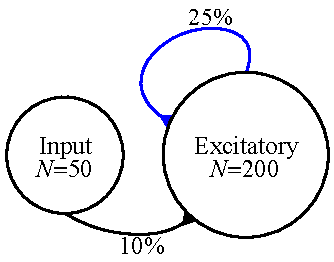
\includegraphics[width=\linewidth]{methods/network_model}
        \caption{}
        \label{figs:methods:network}
    \end{minipage}%
\setcounter{figure}{1}
\setcounter{subfigure}{1}
    \begin{minipage}[b]{0.32\textwidth}
        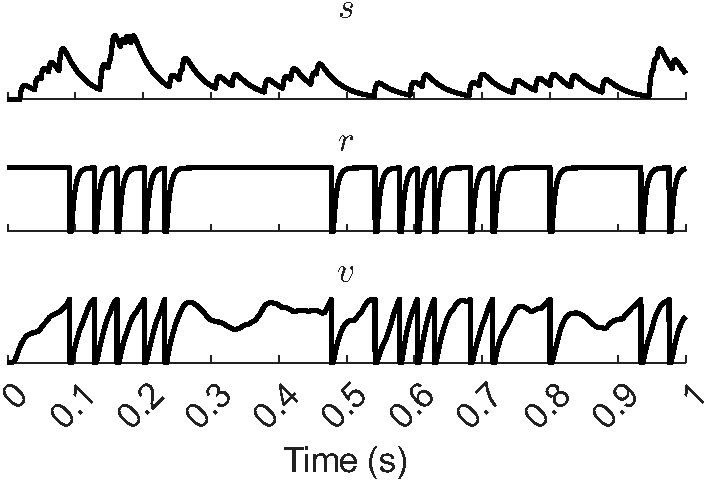
\includegraphics[width=\linewidth]{methods/neurons_and_synapses}
        \caption{}
        \label{figs:methods:neurons_and_synapses}
    \end{minipage}%
\setcounter{figure}{1}
\setcounter{subfigure}{2}
    \begin{minipage}[b]{0.25\textwidth}
        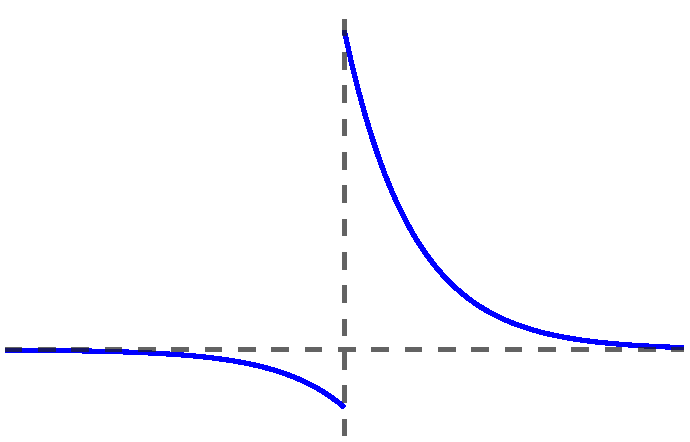
\includegraphics[width=\linewidth]{methods/STDP}
        \caption{}
        \label{figs:methods:STDP}
    \end{minipage}%
\setcounter{figure}{1}
\setcounter{subfigure}{3}
    \begin{minipage}[b]{0.32\textwidth}
        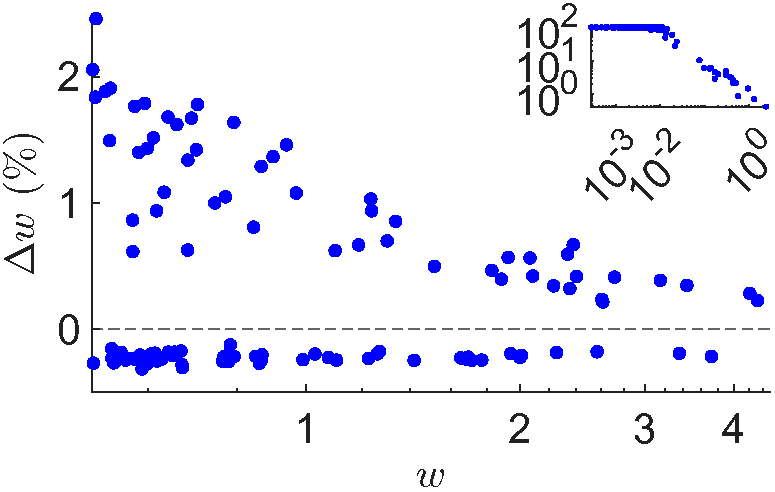
\includegraphics[width=\linewidth]{methods/dependence}
        \caption{}
        \label{figs:methods:weight_dependence}
    \end{minipage}%
\setcounter{figure}{1}
\setcounter{subfigure}{4}
    \begin{minipage}[b]{0.49\textwidth}
        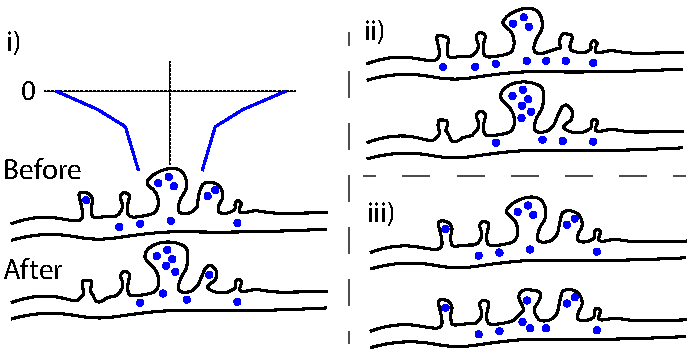
\includegraphics[width=\linewidth]{methods/heterosynaptic_plasticity_model}
        \caption{}
        \label{figs:methods:rbSTDP}
    \end{minipage}%
\setcounter{figure}{1}
\setcounter{subfigure}{5}
    \begin{minipage}[b]{0.4\textwidth}
        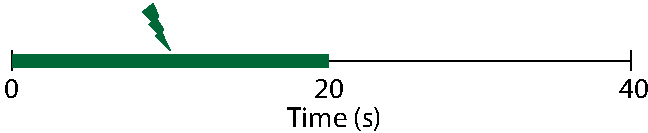
\includegraphics[width=\linewidth]{methods/stimulation_protocol}
        \caption{}
        \label{figs:methods:stimulation_protocol}
    \end{minipage}%
\setcounter{figure}{1}
\setcounter{subfigure}{-1}
    \caption{Network, neuron, and synaptic models and stimulation protocol. {\textbf{(A)}} A pool of \SI{200} excitatory neurons receive input from \SI{50} independent Poisson processes. All recurrent synapses undergo STDP. \textbf{(B)} A synaptic input, $s$, and one neuron's refractoriness, $r$, and membrane potential, $v$. \textbf{(C)} STDP learning window. \textbf{(D)} Synaptic change dependence on weight. \textbf{(E)} Three different scenarios for heterosynaptic plasticity: i) potentiation accompanied by heterosynaptic depression of resources (blue circles) from neighbors, ii) potentiation with resources from the pool, and iii) depression. \textbf{(F)} Input is provided for the first \SI{20}{\second}.}
    \label{figs:methods}
\end{subfigure}

\begin{subfigure}
\setcounter{figure}{2}
\setcounter{subfigure}{0}
    \centering
    \begin{minipage}[b]{0.32\textwidth}
        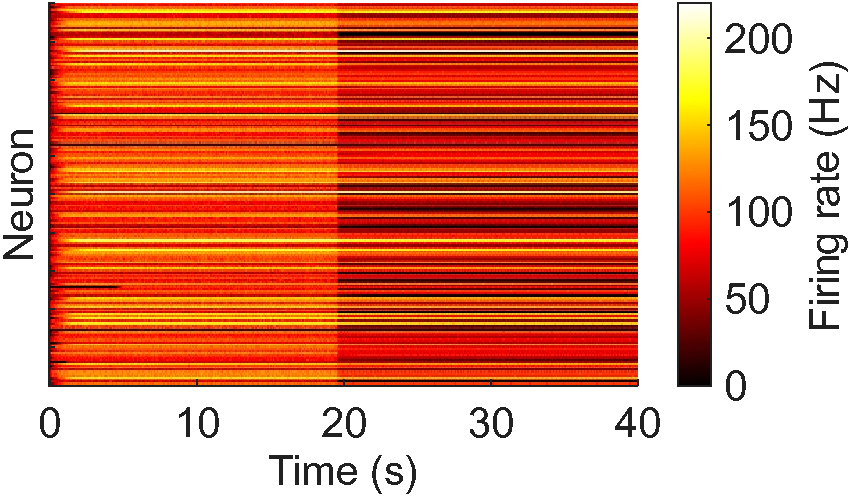
\includegraphics[width=\linewidth]{rbSTDP/Hz}
        \caption{}
        \label{figs:results:firing_rate}
    \end{minipage}%
\setcounter{figure}{2}
\setcounter{subfigure}{1}
    \centering
    \begin{minipage}[b]{0.32\textwidth}
        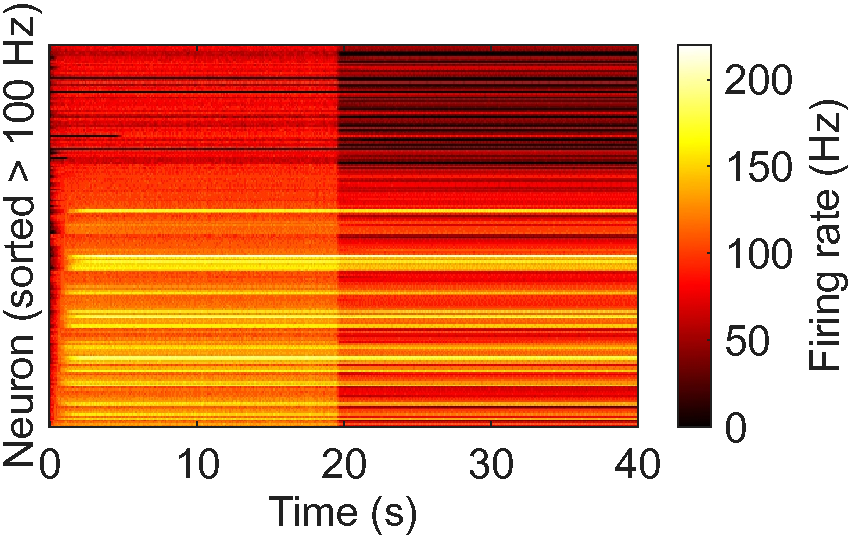
\includegraphics[width=\linewidth]{rbSTDP/Hz_sorted}
        \caption{}
        \label{figs:results:firing_rate_sorted}
    \end{minipage}%
\setcounter{figure}{2}
\setcounter{subfigure}{2}
    \centering
    \begin{minipage}[b]{0.32\textwidth}
        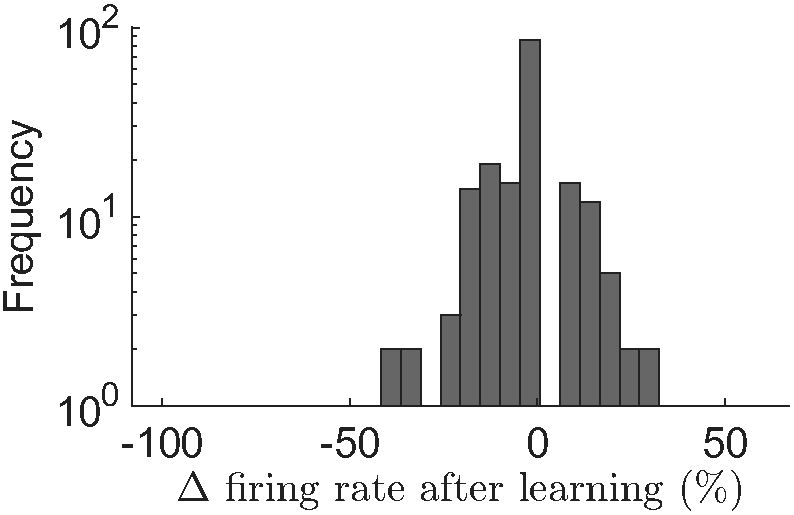
\includegraphics[width=\linewidth]{rbSTDP/Hz_change_histogram}
        \caption{}
        \label{figs:results:firing_rate_change}
    \end{minipage}%
\setcounter{figure}{2}
\setcounter{subfigure}{3}
    \begin{minipage}[b]{0.32\textwidth}
        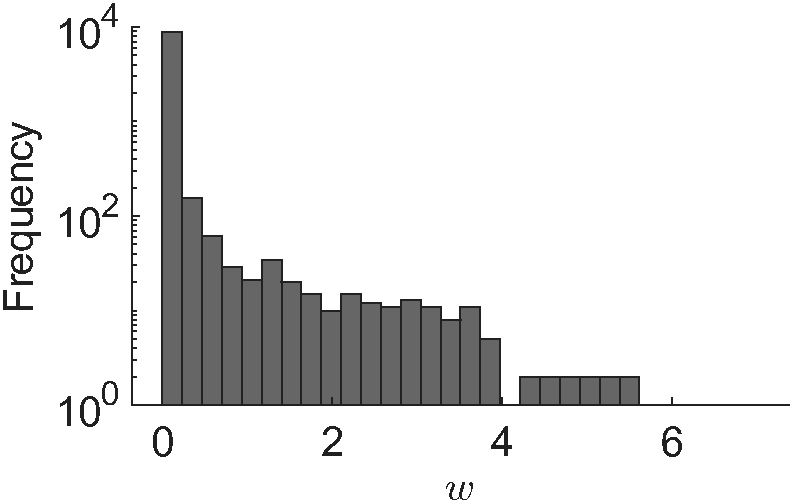
\includegraphics[width=\linewidth]{rbSTDP/weights_E2E_histogram}
        \caption{}
        \label{figs:results:weight_distribution}
    \end{minipage}%
\setcounter{figure}{2}
\setcounter{subfigure}{4}
    \begin{minipage}[b]{0.32\textwidth}
        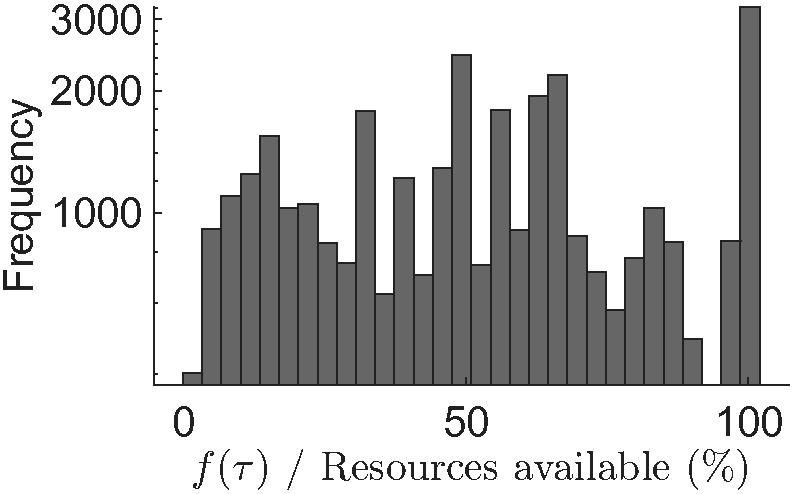
\includegraphics[width=\linewidth]{rbSTDP/non_potentiable_histogram}
        \caption{}
        \label{figs:results:non_potentiable}
    \end{minipage}%
\setcounter{figure}{2}
\setcounter{subfigure}{5}
    \begin{minipage}[b]{0.32\textwidth}
        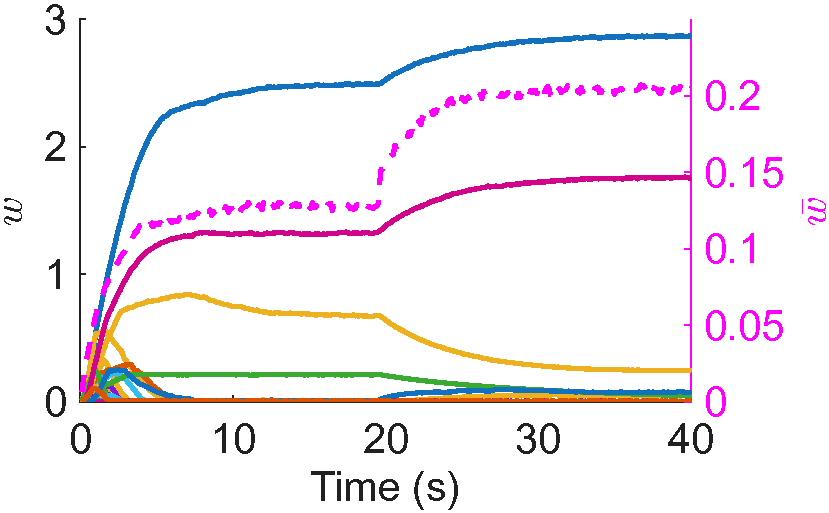
\includegraphics[width=\linewidth]{rbSTDP/weights_E2E_traces}
        \caption{}
        \label{figs:results:weights_traces}
    \end{minipage}%
\setcounter{figure}{2}
\setcounter{subfigure}{6}
    \begin{minipage}[b]{0.32\textwidth}
        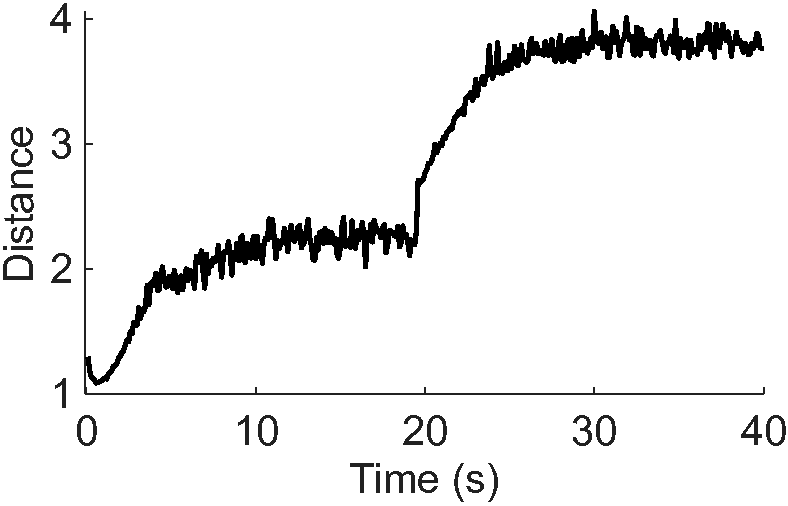
\includegraphics[width=\linewidth]{rbSTDP/weights_E2E_distance}
        \caption{}
        \label{figs:results:weights_distance}
    \end{minipage}%
\setcounter{figure}{2}
\setcounter{subfigure}{7}
    \begin{minipage}[b]{0.32\textwidth}
        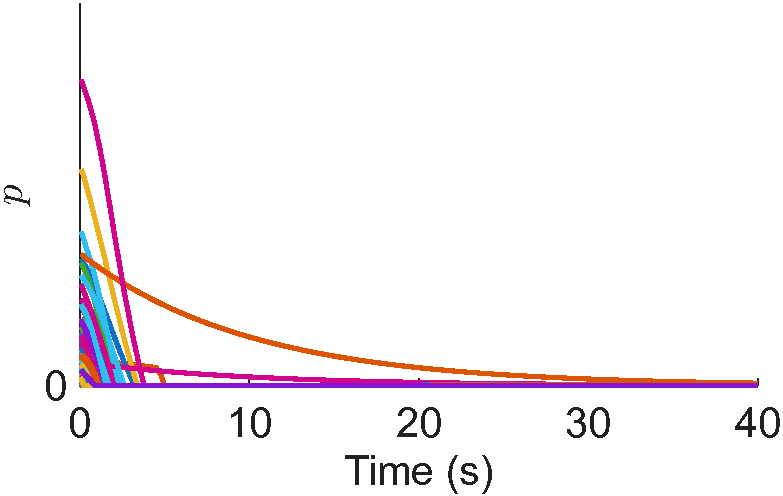
\includegraphics[width=\linewidth]{rbSTDP/resource_pools}
        \caption{}
        \label{figs:results:resource_pools}
    \end{minipage}%
\setcounter{figure}{2}
\setcounter{subfigure}{8}
    \centering
    \begin{minipage}[b]{0.32\textwidth}
        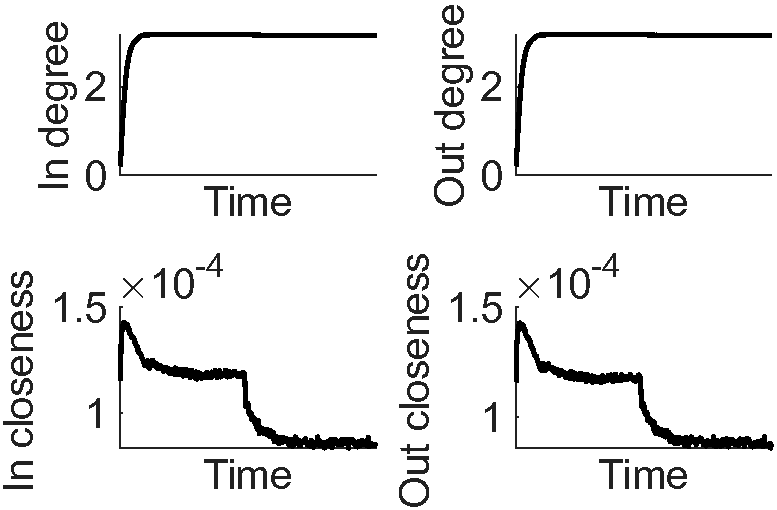
\includegraphics[width=\linewidth]{rbSTDP/digraph_measures_1.pdf}
        \caption{}
        \label{figs:results:centrality}
    \end{minipage}%   
\setcounter{figure}{2}
\setcounter{subfigure}{9}
    \centering
    \begin{minipage}[b]{0.21\textwidth}
        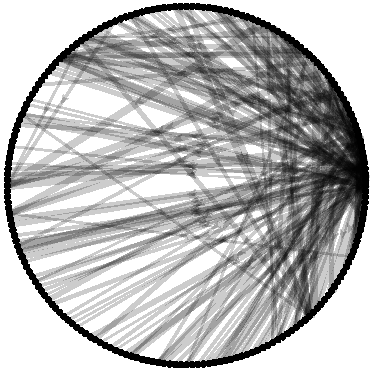
\includegraphics[width=\linewidth]{rbSTDP/digraph_after_learning.pdf}
        \caption{}
        \label{figs:results:network_after_learning}
    \end{minipage}%   
\setcounter{figure}{2}
\setcounter{subfigure}{10}
    \centering
    \begin{minipage}[b]{0.32\textwidth}
        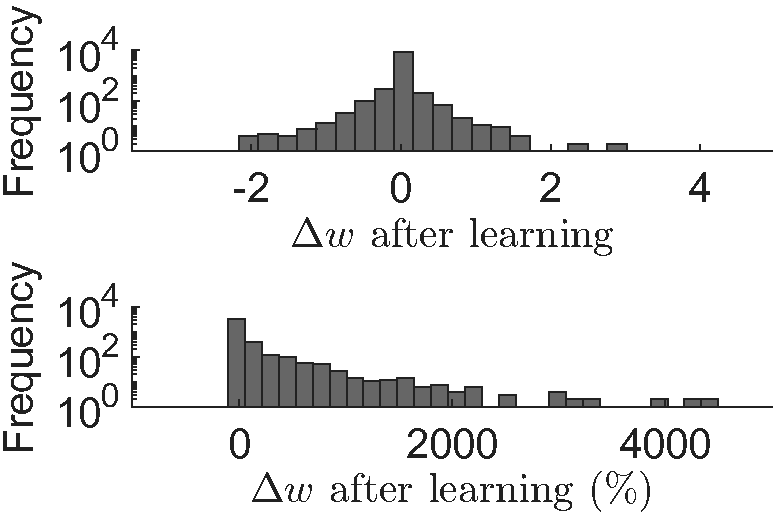
\includegraphics[width=\linewidth]{rbSTDP/weights_E2E_change_histogram.pdf}
        \caption{}
        \label{figs:results:network_change}
    \end{minipage}%   
\setcounter{figure}{2}
\setcounter{subfigure}{11}
    \centering
    \begin{minipage}[b]{0.21\textwidth}
        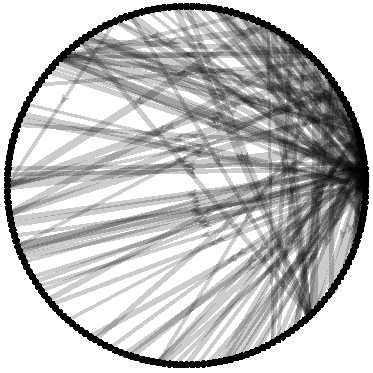
\includegraphics[width=\linewidth]{rbSTDP/digraph_end.pdf}
        \caption{}
        \label{figs:results:network_end}
    \end{minipage}%   
\setcounter{figure}{2}
\setcounter{subfigure}{-1}
    \caption{Typical network dynamics. {\textbf{(A)}} Firing rates of the network's neurons. {\textbf{(B)}} Sorted firing rate of the network's neurons for when they first fire $\ge\SI{100}{\hertz}$. {\textbf{(C)}} Change in the firing rate from after learning to the end of the simulation. {\textbf{(D)}} Weights, $w$, after learning. {\textbf{(E)}} Left axis: Example of \SI{100}{} synapses' weights. Right axis/dashed line: Mean of nonfilopodia synapses' weights. {\textbf{(C)}} Distance between nonfilopodia spines. {\textbf{(D)}}  {\textbf{(E)}} Resource pools, $p$. {\textbf{(F)}} Mean in degree, out degree, in closeness, and out closeness during the simulation. {\textbf{(G)}} Network of neurons after learning. Only the strongest \SI{10}{\percent} are shown. Line width represents weight. {\textbf{(H)}} Weight change after learning. {\textbf{(I)}} Network of neurons at the end of the simulation.}
    \label{figs:results:typical}
\end{subfigure}

\begin{subfigure}
\setcounter{figure}{3}
\setcounter{subfigure}{0}
    \begin{minipage}[b]{0.32\textwidth}
        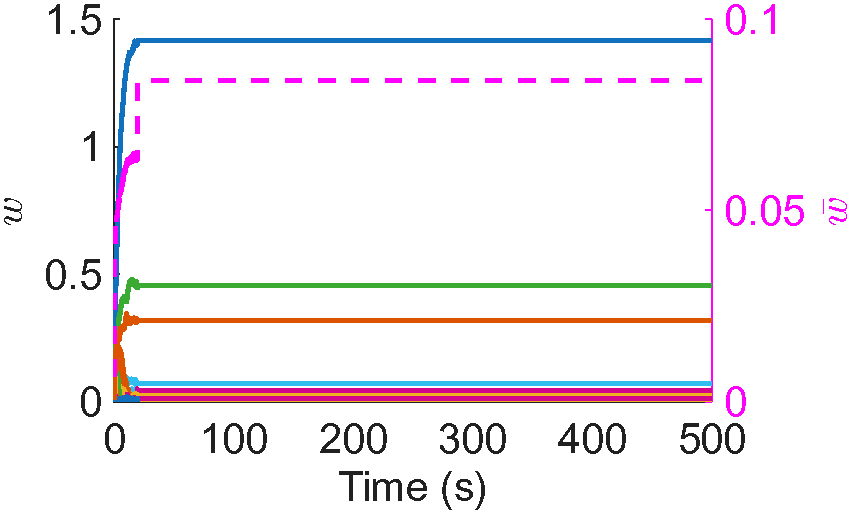
\includegraphics[width=\linewidth]{rbSTDP_long/weights_E2E_traces.pdf}
    \end{minipage}%

\setcounter{figure}{3}
\setcounter{subfigure}{-1}
    \caption{Example of \SI{100}{} synapses' weights during a long simulation.}
    \label{figs:results:long}
\end{subfigure}

\begin{subfigure}
\setcounter{figure}{4}
\setcounter{subfigure}{0}
    \begin{minipage}[b]{0.4\textwidth}
        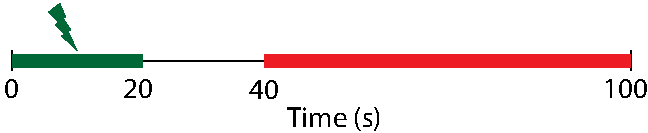
\includegraphics[width=\linewidth]{AD/stimulation_protocol_AD}
        \caption{}
        \label{figs:results:AD:stimulation_protocol}
    \end{minipage}%
\setcounter{figure}{4}
\setcounter{subfigure}{1}
    \begin{minipage}[b]{0.32\textwidth}
        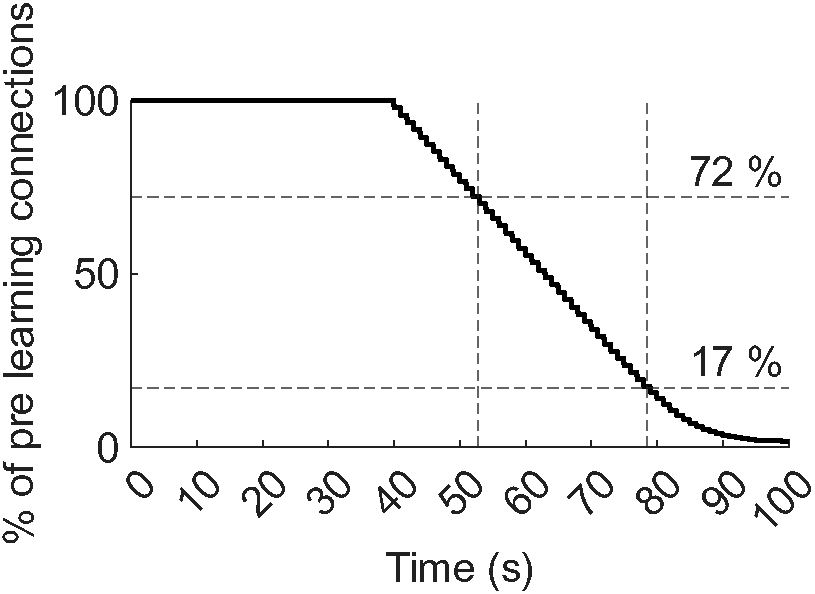
\includegraphics[width=\linewidth]{AD/connections}
        \caption{}
        \label{figs:results:AD:connections}
    \end{minipage}%
\setcounter{figure}{4}
\setcounter{subfigure}{2}
    \centering
    \begin{minipage}[b]{0.32\textwidth}
        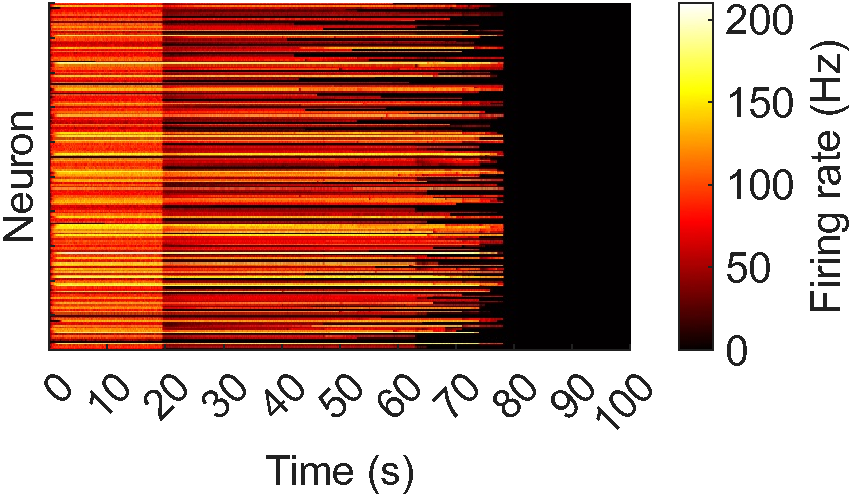
\includegraphics[width=\linewidth]{AD/Hz}
        \caption{}
        \label{figs:results:AD:firing_rate}
    \end{minipage}%
\setcounter{figure}{4}
\setcounter{subfigure}{3}
    \centering
    \begin{minipage}[b]{0.32\textwidth}
        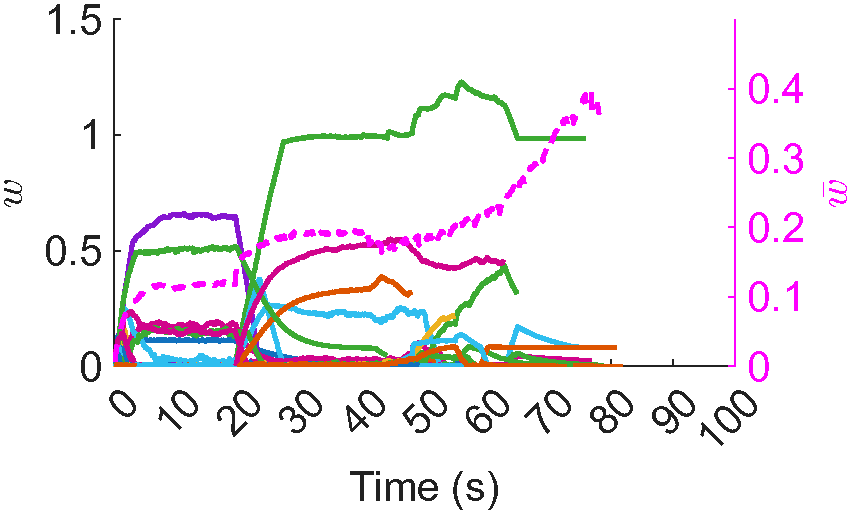
\includegraphics[width=\linewidth]{AD/weights_E2E_traces}
        \caption{}
        \label{figs:results:AD:weights_traces}
    \end{minipage}%
\setcounter{figure}{4}
\setcounter{subfigure}{4}
    \centering
    \begin{minipage}[b]{0.32\textwidth}
        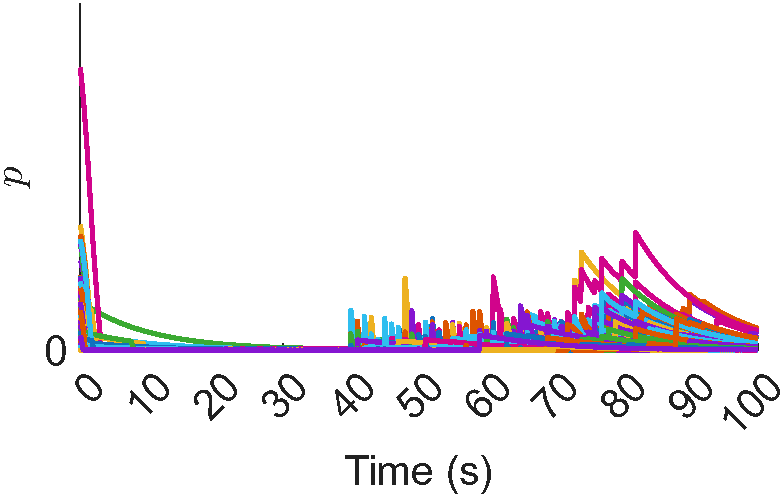
\includegraphics[width=\linewidth]{AD/resource_pools}
        \caption{}
        \label{figs:results:AD:resource_pools}
    \end{minipage}%
\setcounter{figure}{4}
\setcounter{subfigure}{5}
    \begin{minipage}[b]{0.32\textwidth}
        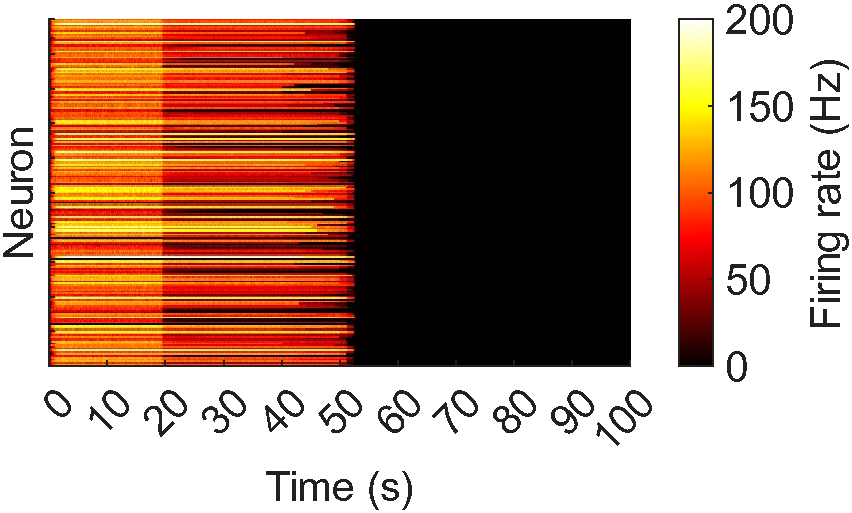
\includegraphics[width=\linewidth]{AD/Hz_no_resources}
        \caption{}
        \label{figs:results:AD:Hz_no_resources}
    \end{minipage}%
\setcounter{figure}{4}
\setcounter{subfigure}{6}
    \begin{minipage}[b]{0.32\textwidth}
        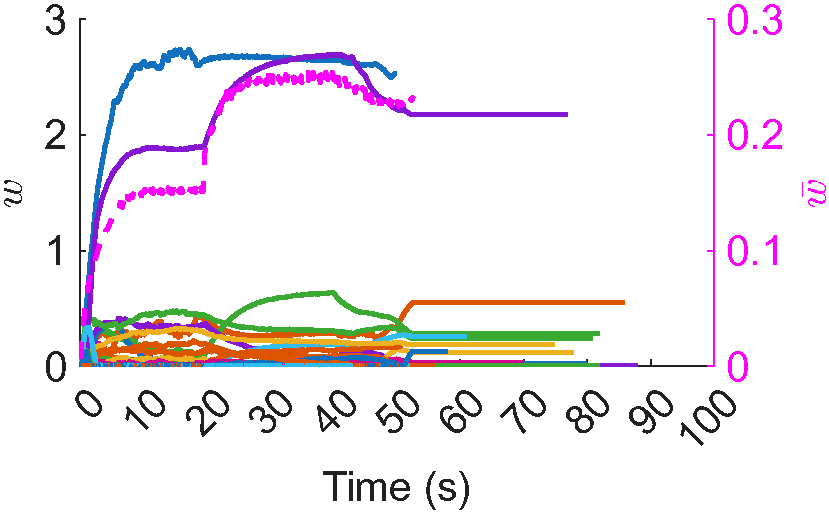
\includegraphics[width=\linewidth]{AD/weights_E2E_traces_no_resources}
        \caption{}
        \label{figs:results:AD:weights_traces_no_resources}
    \end{minipage}%
\setcounter{figure}{4}
\setcounter{subfigure}{7}
    \begin{minipage}[b]{0.32\textwidth}
        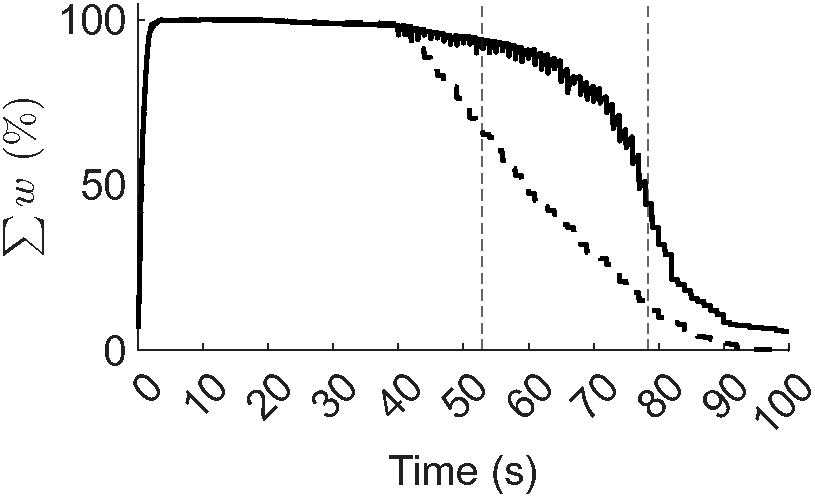
\includegraphics[width=\linewidth]{AD/weights_E2E_sum}
        \caption{}
        \label{figs:results:AD:weights_sums}
    \end{minipage}%
\setcounter{figure}{4}
\setcounter{subfigure}{8}
    \begin{minipage}[b]{0.32\textwidth}
        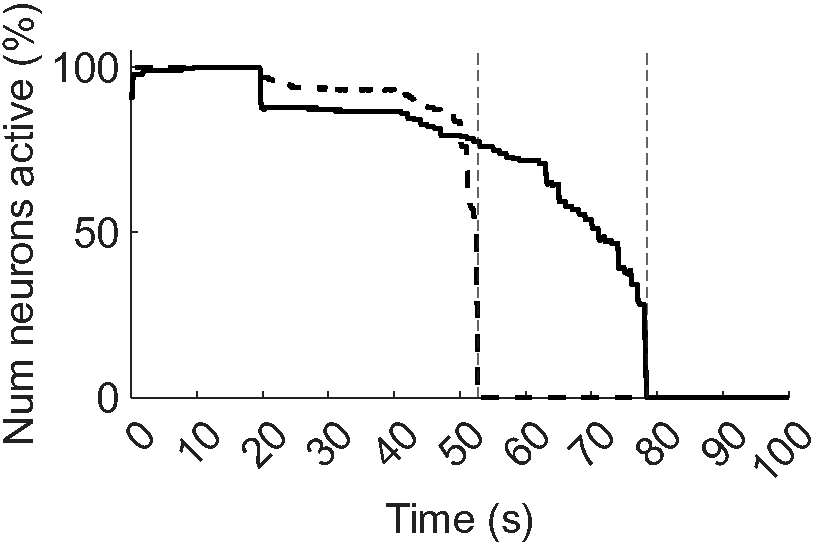
\includegraphics[width=\linewidth]{AD/Hz_sum}
        \caption{}
        \label{figs:results:AD:Hz_sums}
    \end{minipage}%
\setcounter{figure}{4}
\setcounter{subfigure}{-1}
    \caption{Typical network dynamics with and without resource pool replenishment while removing connections. \textbf{(A)} Input is provided for the first \SI{20}{\second}. Synapses are progressively deleted from \SI{40}{\second} on (red). {\textbf{(B)}} Progressive synaptic loss. {\textbf{(C)}} Firing rates of the network's neurons with replenishment of the resource pool. {\textbf{(D)}} Left axis: Example of \SI{100}{} synapses' weights with resource pool replenishment. Right axis/dashed line: Mean of nonfilopodia synapses' weights. {\textbf{(E)}} Resource pools, $p$, with replenishment of the resource pool. {\textbf{(F)}} Firing rates of the network's neurons without replenishment of the resource pool. {\textbf{(G)}} Left axis: Example of \SI{100}{} synapses' weights without replenishment of the resource pool. Right axis/dashed line: Mean of nonfilopodia synapses' weights. {\textbf{(H)}} Sum of weights as a percentage of the maximum sum of weights. Solid line, with resource replenishment; dashed line, without resource replenishment. {\textbf{(I)}} The number of active neurons as a percentage of the maximum number of active neurons. Solid line, with resource replenishment; dashed line, without resource replenishment. {\textbf{(B)}}, {\textbf{(H)}}, and {\textbf{(I)}} Vertical lines are when all neurons stopped firing either with or without resource replenishment. {\textbf{(D)}} and {\textbf{(G)}} Weights are shown while they exist and the mean of nonfilopodia synapses' weights is shown while neurons are active.}
    \label{figs:results:AD}
\end{subfigure}

%%% If you don't add the figures in the LaTeX files, please upload them when submitting the article.
%%% Frontiers will add the figures at the end of the provisional pdf automatically
%%% The use of LaTeX coding to draw Diagrams/Figures/Structures should be avoided. They should be external callouts including graphics.

\end{document}